\section{微积分基本定理 - revisited - 下}\label{032}

\subsection{散度定理}

散度定理又叫做\textbf{高斯定理} (Gauss's theorem), in which \[
\boxed{\oiint\boldsymbol{v}\cdot\mathrm{d}\boldsymbol{a}=\iiint\nabla\cdot\boldsymbol{v}\ \mathrm{d}V},
\] 即在一闭合区域内, 【其边界所对应的闭合曲面上的, 这个向量场的面积分】,
等于【对一个向量场的散度的体积分】.

证明思路和格林定理的味道很像,
事实上散度定理确实可以看作是二维的格林定理法形式或者通量形式
(参见【\ref{031}\nameref{031}】) 在三维的推广.

首先, 面积分 $\oiint\boldsymbol{v}\cdot\mathrm{d}\boldsymbol{a}$
可以''拆解''成许多个小的体积表面上的积分之和 (如下图所示),
因为通量积分是定向的, 所以重复计算的部分会因为方向不同而抵消.
现在关注一块小的体积表面上的积分, 方便起见,
将小的体积定为棱平行于坐标轴的一个立方体, 这样一来, 积分
$\oiint\boldsymbol{v}\cdot\mathrm{d}\boldsymbol{a}$
可以大致分成三个方向上的积分: 上-下面、左-右面、前-后面.

\begin{tcolorbox}[size=fbox, breakable, enhanced jigsaw]
    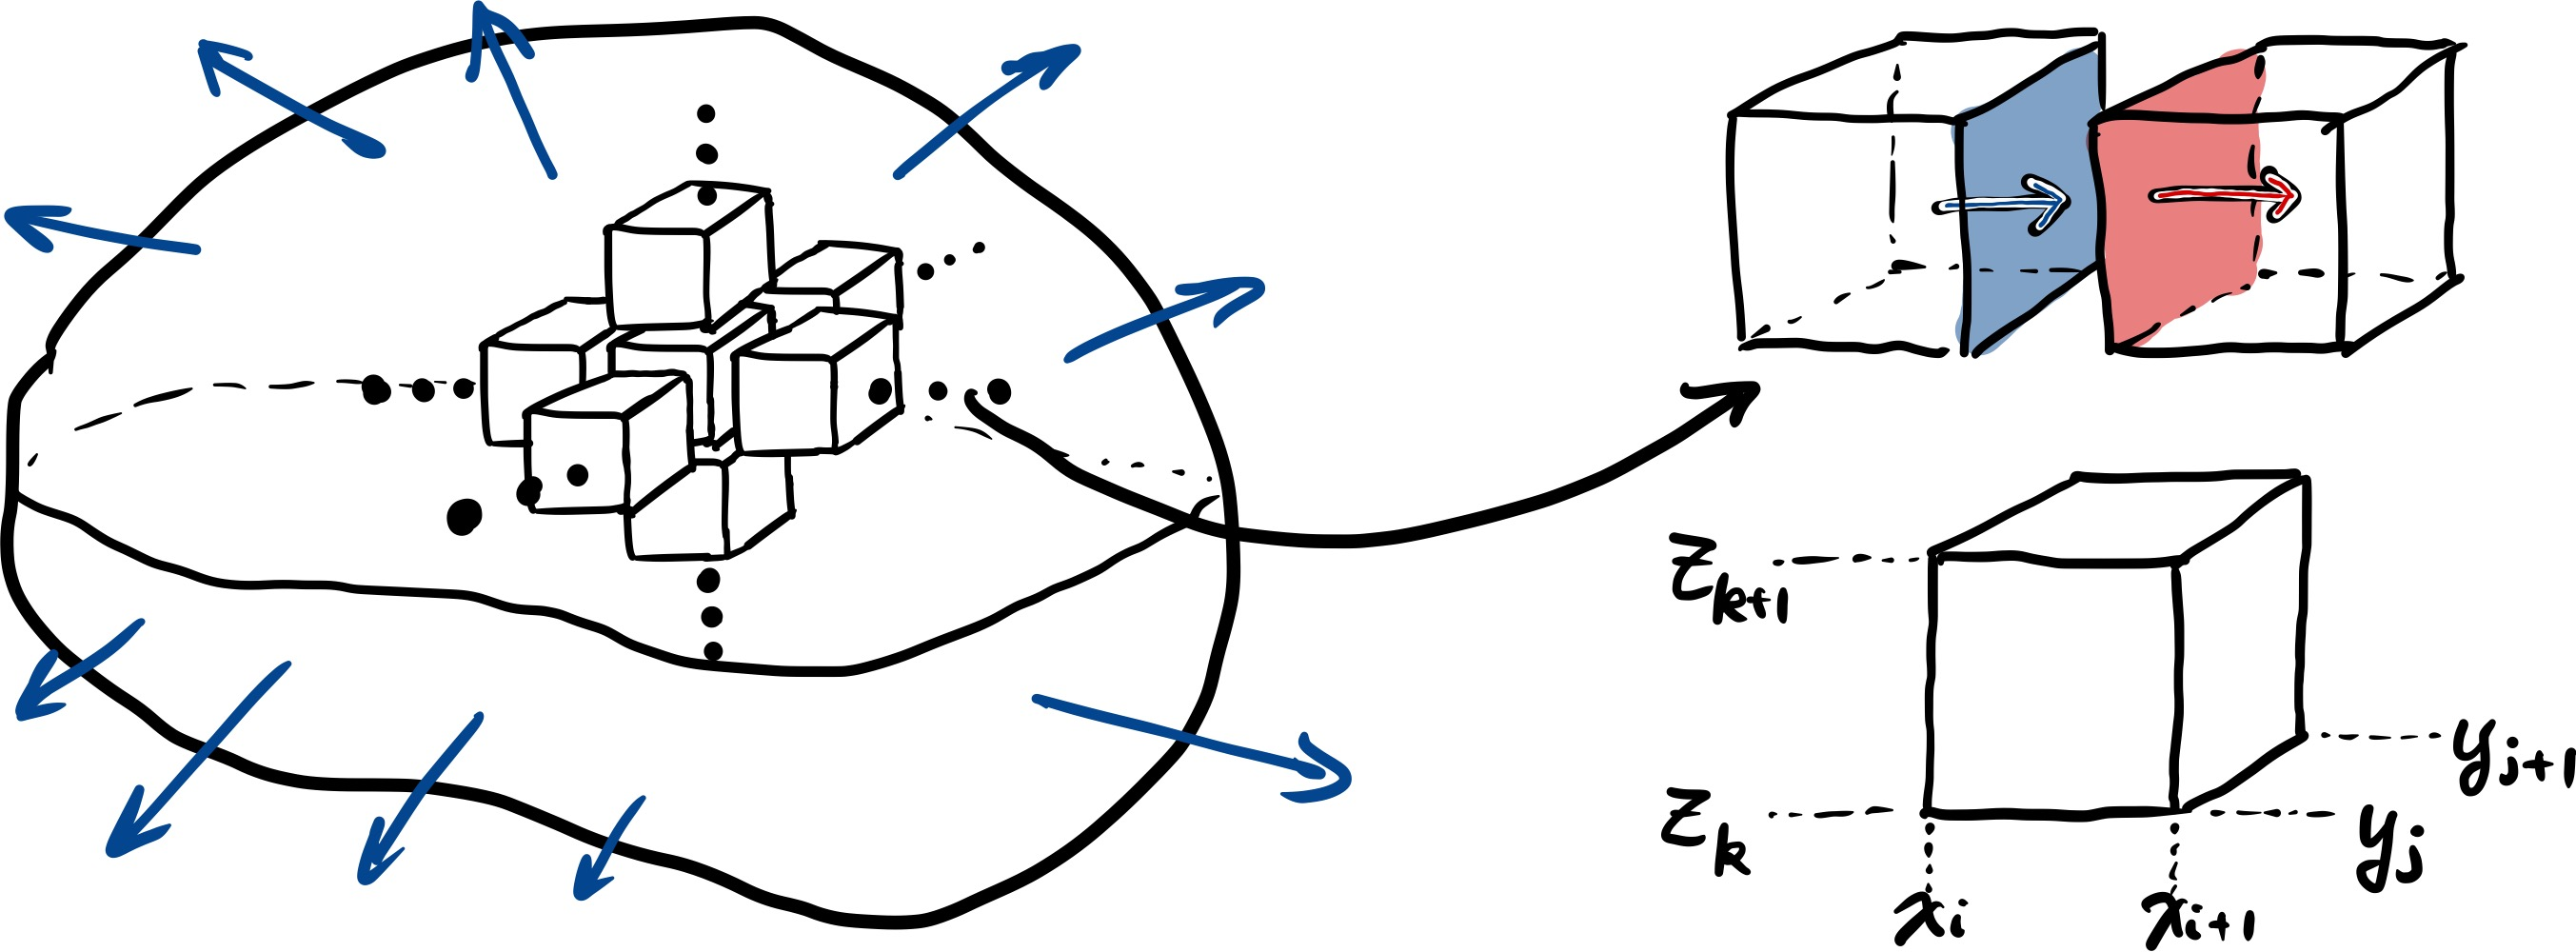
\includegraphics[width=0.9\textwidth]{./img/image-20240618231420999.png}
\end{tcolorbox}

以上-下面上的通量积分为例, 在一块小的体积上, 它应该为 \[
v_z\big|_{z=z_{k+1}}\cdot(y_{j+1}-y_{j})\cdot(x_{i+1}-x_i)-v_z\big|_{z=z_{k}}\cdot(y_{j+1}-y_{j})\cdot(x_{i+1}-x_i),
\] 这里 $v_z$ 代表向量场 $\boldsymbol{v}$ 平行于 $z$-轴的分量,
即有 \[\boldsymbol{z}=v_x\hat{\imath}+v_y\hat{\jmath}+v_z\hat{k}\].

\begin{newquote}
另外, 在 evaluate $v_z$ 时, 我们忽略代入不同的 $x$ 和 $y$ 的影响,
只考虑 $z$ 值不同导致 $v_z$ 的变化; 但实际上 $x$ 和 $y$
的取值当然会影响 $v_z(x,y,z)$, 尤其是在一个有限的平面上,
但是稍后我们就会将我们所关注的小立方的体积推至无穷小,
这样它的各个表面也会变得无穷小, $v_z$ 的取值也缩到某个固定的 $x$ 和
$y$ 上了.
\end{newquote}

然后利用微积分基本定理 (回顾【\ref{031}\nameref{031}】开头), 会有上-下面上的通量积分为 \[
\int_{z_k}^{z_{k+1}}\frac{\partial v_z}{\partial z}\mathrm{d}z\Delta x\Delta y,
\] 这里 $\Delta x=(x_{i+1}-x_i)$, $\Delta y=(y_{j+1}-y_{j})$.
当我们将小立方变为一个体积微元, 即取 $\Delta x\rightarrow \mathrm{d}x$
以及 $\Delta y\rightarrow\mathrm{d}y$, 它上-下面的通量微元变为 \[
\frac{\partial v_z}{\partial z}\mathrm{d}z\mathrm{d}x\mathrm{d}y.
\] 类似的, 左-右面和前-后面的通量微元分别应为 \[
\frac{\partial v_x}{\partial x}\mathrm{d}x\mathrm{d}y\mathrm{d}z,\frac{\partial v_y}{\partial y}\mathrm{d}x\mathrm{d}y\mathrm{d}z.
\] 整个体积微元表面上的通量之和便是 \[
\left(\frac{\partial v_x}{\partial x}+\frac{\partial v_y}{\partial y}+\frac{\partial v_z}{\partial z}\right)\mathrm{d}x\mathrm{d}y\mathrm{d}z.
\] 这样一来, 一个有限的体积表面上的通量, 例如先前考虑的小立方体, 应为 \[
\int_{z_k}^{z_{k+1}}\int_{y_j}^{y_{j+1}}\int_{x_i}^{x_{i+1}}\left(\frac{\partial v_x}{\partial x}+\frac{\partial v_y}{\partial y}+\frac{\partial v_z}{\partial z}\right)\mathrm{d}x\mathrm{d}y\mathrm{d}z.
\] 继而小立方所构成的整个体积表面上的通量就是 \[
\begin{aligned}
&\oiint\boldsymbol{v}\cdot\mathrm{d}\boldsymbol{a}\\
=&\sum_{i,j,k}\int_{z_k}^{z_{k+1}}\int_{y_j}^{y_{j+1}}\int_{x_i}^{x_{i+1}}\left(\frac{\partial v_x}{\partial x}+\frac{\partial v_y}{\partial y}+\frac{\partial v_z}{\partial z}\right)\mathrm{d}x\mathrm{d}y\mathrm{d}z\\
=&\iiint\left(\frac{\partial v_x}{\partial x}+\frac{\partial v_y}{\partial y}+\frac{\partial v_z}{\partial z}\right)\mathrm{d}x\mathrm{d}y\mathrm{d}z.
\end{aligned}
\] 不难发现, 最后一行括号内的项实际上就是 $\boldsymbol{v}$ 的散度
$\nabla\cdot\boldsymbol{v}$, 于是证毕.

\subsection{旋度定理}

旋度定理又叫做\textbf{斯托克斯定理} (Stokes' theorem), \[
\boxed{\oint\boldsymbol{v}\cdot\mathrm{d}\boldsymbol{r}=\iint\nabla\times\boldsymbol{v}\cdot\mathrm{d}\boldsymbol{a}},
\] 即在一个曲面上, 【其边界, 也就是一个闭合曲线上的一个向量场的线积分】,
等于【这个向量场的旋度在这个曲面上的面积分】.

证明思路和格林定理的味道还是很像,
而且事实上旋度定理又是二维的格林定理切形式或者环量形式 (参见【\ref{031}\nameref{031}】)
在三维的推广.

假设有一简单曲面, 选取一个合适的坐标系, 使得其可以被表示为 $z(x,y)$
的形式,

\begin{tcolorbox}[size=fbox, breakable, enhanced jigsaw]
    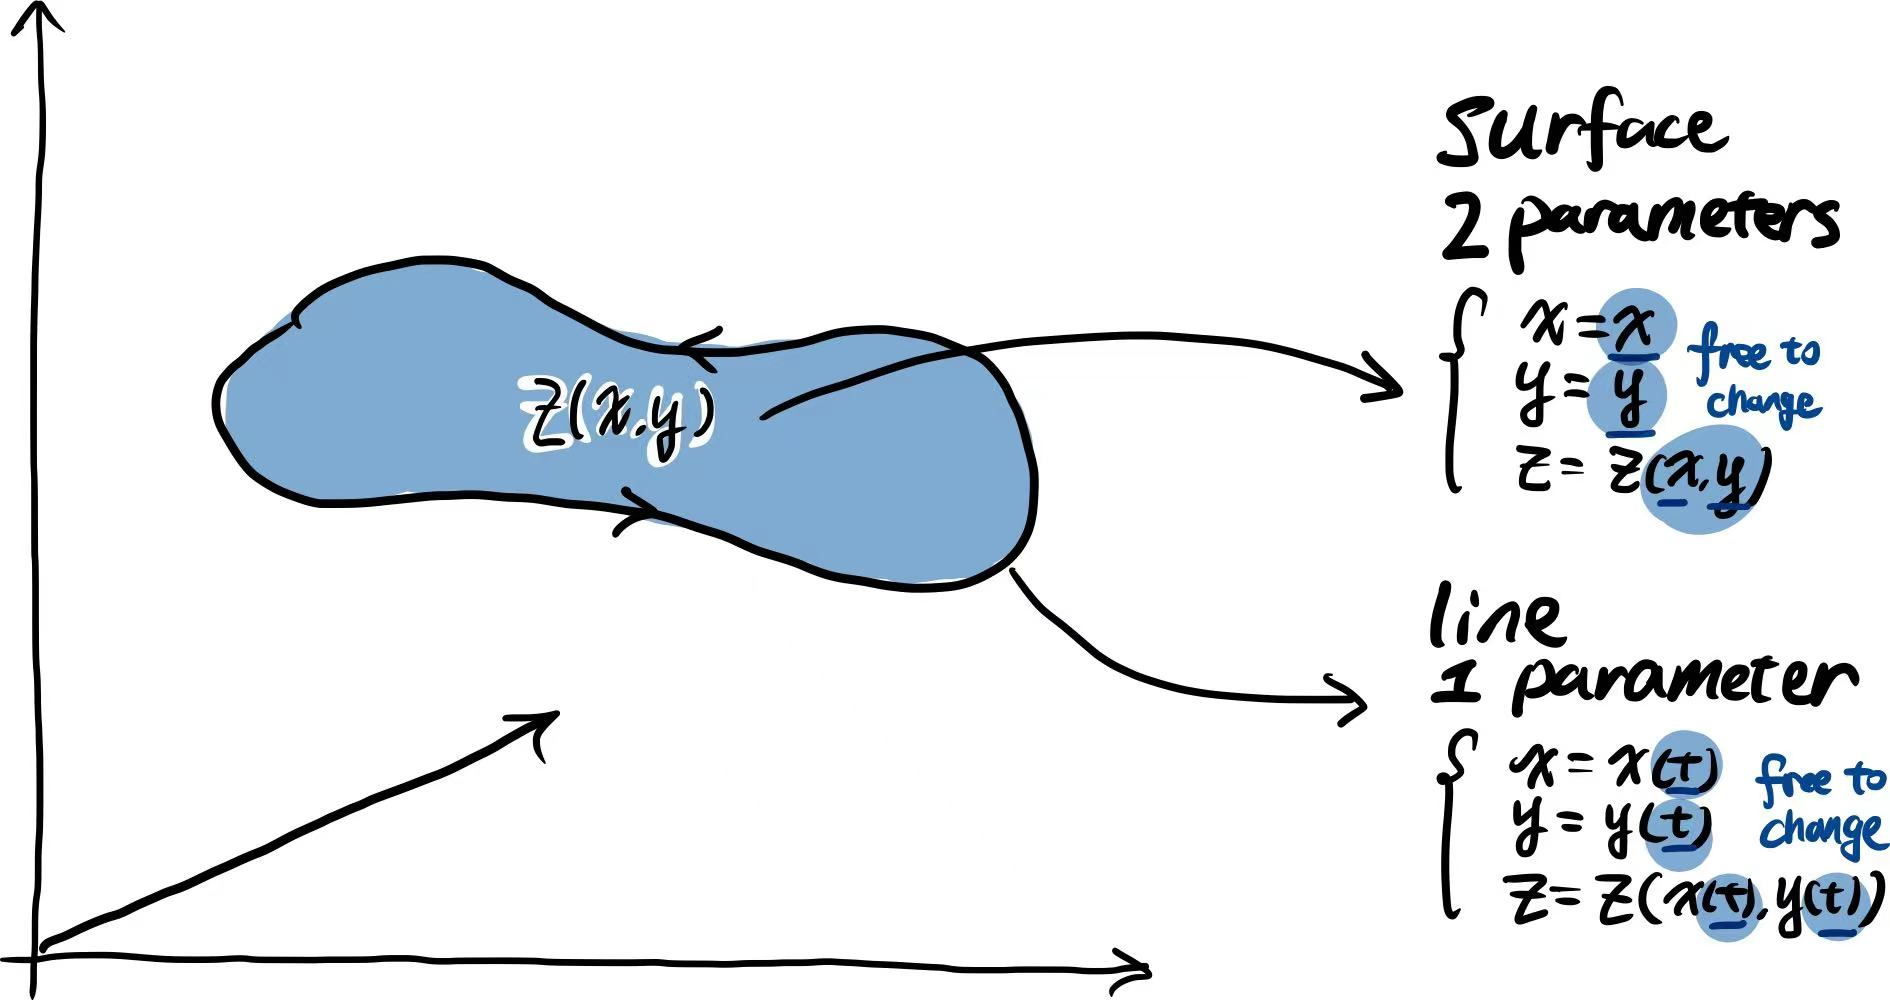
\includegraphics[width=0.9\textwidth]{./img/image-20240621050652898.png}
\end{tcolorbox}

\begin{newquote}
即给定某个 $(x,y)$ 位置, 这个平面的高度 $z$ 可以被确定;
当然旋转坐标轴, 用类似 $x(y,z)$ 的形式表示也完全没问题;
甚至可以利用参数化 (parametrization), 因为一个平面是二维的,
所以两个自由度就可以确定一个平面, 选定参数$\{s,t\}$,
平面还可以表示为形如 \[
\begin{cases}
x(s,t)\\
y(s,t)\\
z(s,t)
\end{cases}
\] 的参数化平面.
\end{newquote}

因为这个平面是二维的, 所以这个平面上某点的切向量是无限多的,
但是我们可以选定两个基向量 (复习【\ref{025}\nameref{025}】),
然后其他的向量便可以由这两个基向量张 (span) 成. 在【\ref{030}\nameref{030}】的线积分中,
我们提到过 $\mathrm{d}\boldsymbol{r}$ 的几何含义应该是曲线的切向量,
那么推广到曲面上, 切向量的基向量比较''自然''的选择便是
$1\hat{\imath}+0\hat{\jmath}+(\partial z/\partial x)\hat{k}$ 和
$0\hat{\imath}+1\hat{\jmath}+(\partial z/\partial y)\hat{k}$.

\begin{newquote}
这看起来一点都不''自然''. 这里''简单''且不严格地扩充一下,
来一个''天地联通'':

地: 比较接地气的铺垫, 我们在看多元函数的变化率时 (复习【\ref{023}\nameref{023}】),
因为函数时关于多个变量的, 在某个取值下, 函数并没有''唯一''的变化率; 比如
$f(x,y)$, 在某个特定的点 $(x,y)$ 上, $f$ 的变化率并不唯一, 最沿着
$x$ 的方向上它有一个变化率, 沿着 $y$ 的方向上有另一个变化率, 沿着
$y=x$ 的方向上还有一个不同的变化率; 为此, 只有声明好一个特定的方向,
才有一个唯一的变化率, 这样的变化率用\textbf{方向导数} (directional
derivative) 来给出, 方向的声明通常经由一个 (单位) 向量
$\boldsymbol{v}$ 给出,
然后一个多元函数的方向导数便可以表示为这个函数的梯度点乘上这个向量,
i.e.~$\nabla f\cdot\boldsymbol{v}$, (回顾【\ref{028}\nameref{028}】提及的梯度下降法).
若将函数 $f$ 看作一个平面, 那么梯度 $\nabla f$
可以视作一个特殊的切于这个平面的向量, 它所在的方向变化率最大, in
general, 偏导这个操作似乎是给出了平行于某个坐标轴的切向量.

天: (剧透警告) 既然偏导这个操作可以给出切向量, 在\textbf{微分几何}
(differential geometry) 中, 给一个流形上某点的领域选定坐标系,
该点处的所有切向量可以被 $\{\partial/\partial_{x_n}\}$ 线性表出
(即任意切向量 $\boldsymbol{T}$ 可以展开成
$\boldsymbol{T}=\sum_na_n\partial/\partial_{x_n}$, $a_n$ 是分量,
$\partial/\partial_{x_n}$ 充当基底, 回顾【\ref{024}\nameref{024}】文末的讨论),
(当然这个表示其实省略了偏导要作用在一个对象上,
类似这种省略作用对象的标记在很多场合常有出现).

因为现在我们的平面用参数化地视角看是 \[
\begin{cases}
x=x\\
y=y\\
z=z(x,y)
\end{cases}
\] 其中 $\{x,y\}$ 可以看作参数, 于是 $\partial/\partial_{x}$ 和
\[\partial/\partial_{y}\] 对应的两个基向量便是 \[
\begin{aligned}
\boldsymbol{T}_1=\frac{\partial}{\partial x}\left(x\hat{\imath}+y\hat{\jmath}+z(x,y)\hat{k}\right)&=1\hat{\imath}+0\hat{\jmath}+\frac{\partial z}{\partial x}\hat{k},\\
\boldsymbol{T}_2=\frac{\partial}{\partial y}\left(x\hat{\imath}+y\hat{\jmath}+z(x,y)\hat{k}\right)&=0\hat{\imath}+1\hat{\jmath}+\frac{\partial z}{\partial y}\hat{k}.
\end{aligned}
\]
\end{newquote}

有了这两个''正交''的切向量之后, 实际上便可确定一个切面,
继而可以利用叉乘, 得到一个垂直于这个切面,
或者说同时垂直于这两个切向量的法向量, 省略一些步骤, 不难得到法向量为 \[
\boldsymbol{n}=\boldsymbol{T}_1\times \boldsymbol{T}_2=-\frac{\partial z}{\partial x}\hat{\imath}-\frac{\partial z}{\partial y}\hat{\jmath}+1\hat{k}.
\] 于是切面上一块面元的方向便可以由这个法向量给出, 即
$\mathrm{d}\boldsymbol{a}=\boldsymbol{n}\mathrm{d}a$. 如此一来,
$\iint\nabla\times\boldsymbol{v}\cdot\mathrm{d}\boldsymbol{a}$
便可写作 \[
\iint\left[-\left(\frac{\partial v_z}{\partial y}-\frac{\partial v_y}{\partial z}\right)\frac{\partial z}{\partial x}-\left(\frac{\partial v_x}{\partial z}-\frac{\partial v_z}{\partial x}\right)\frac{\partial z}{\partial y}+-\left(\frac{\partial v_y}{\partial x}-\frac{\partial v_x}{\partial y}\right)1\right]\mathrm{d}x\mathrm{d}y.\tag{正}
\] 接下来考虑这个曲面的边界, 也就是一个闭合曲线, 曲线是一维的,
所以可以用一个参数来完成参数化, \[
\begin{cases}
x=x(t)\\
y=y(t)\\
z=z(x(t),y(t))
\end{cases}
\] 于是曲线上的切向量 $\mathrm{d}\boldsymbol{r}$, 利用链式规则, 便是
\[
\begin{aligned}
\mathrm{d}\boldsymbol{r}=&\mathrm{d}x\hat{\imath}+\mathrm{d}y\hat{\jmath}+\mathrm{d}z\hat{k}\\
=&\left[\frac{\mathrm{d}x}{\mathrm{d}t}\hat{\imath}+\frac{\mathrm{d}y}{\mathrm{d}t}\hat{\jmath}+\left(\frac{\partial z}{\partial x}\frac{\mathrm{d}x}{\mathrm{d}t}+\frac{\partial z}{\partial y}\frac{\mathrm{d}y}{\mathrm{d}t}\right)\hat{k}\right]\mathrm{d}t.
\end{aligned}
\] 如此一来 $\oint\boldsymbol{v}\cdot\mathrm{d}\boldsymbol{r}$
就可以写作 \[
\begin{aligned}
&\int\left[v_x\frac{\mathrm{d}x}{\mathrm{d}t}+v_y\frac{\mathrm{d}y}{\mathrm{d}t}+v_z\left(\frac{\partial z}{\partial x}\frac{\mathrm{d}x}{\mathrm{d}t}+\frac{\partial z}{\partial y}\frac{\mathrm{d}y}{\mathrm{d}t}\right)\right]\mathrm{d}t\\
=&\int\left[\left(v_x+v_z\frac{\partial z}{\partial x}\right)\frac{\mathrm{d}x}{\mathrm{d}t}+\left(v_y+v_z\frac{\partial z}{\partial y}\right)\frac{\mathrm{d}y}{\mathrm{d}t}\right]\mathrm{d}t\\
=&\oint\left[\left(v_x+v_z\frac{\partial z}{\partial x}\right)\mathrm{d}x+\left(v_y+v_z\frac{\partial z}{\partial y}\right)\mathrm{d}y\right]
\end{aligned}
\] 然后利用微积分基本定理, 将小括号内的项写为其导数被积分的形式, 便有 \[
=\iint\left[\frac{\partial}{\partial y}\left(v_x+v_z\frac{\partial z}{\partial x}\right)\mathrm{d}x\mathrm{d}y+\frac{\partial}{\partial x}\left(v_y+v_z\frac{\partial z}{\partial y}\right)\mathrm{d}y\mathrm{d}x\right].\tag{正}
\] 将偏导作用在小括号内的项上, 并加以整理, 不难得到两个标注 $(\text{正})$
的公式是相等的, 于是证毕.

\begin{newquote}
前面提到过旋度定理是格林定理切形式或者环量形式的推广;
将旋度定理应用到向量场
$\boldsymbol{v}=v_x\hat{\imath}+v_y\hat{\jmath}+0\hat{k}$,
曲面也限制平行于 $x-y$ 面, 这个特殊的 case 便可将旋度定理 reduce
回格林定理切形式或者环量形式, 读者可自行尝试.
\end{newquote}